\section{Introduction}
The annealing is the essential concept of the EAPM.
However, the annealing
is an unstable method
because the obtained solutions cannot be further improved
once the EAPM converges.
This is the problem of local optima.

To overcome this problem,
this paper proposes a novel method, Hierarchical Importance
Sampling (HIS) that can be used instead of the annealing.
The basic principle is to generate multiple sample sets
with different diversities
\footnote{
The exchange Monte Carlo method (EMC) \cite{hukushima:emc}
uses the same concept of sampling from
multiple target distributions with different diversities.
EMC is one of the Markov chain Monte Carlo methods (MCMC) \cite{bishop:ml}.
MCMC and EMC are essentially different from EAPM and HIS.
The relationships among EAPM, MCMC, HIS, and EMC are 
summarized in Section \ref{app-mcmc}.}.
For example, one sample set may be almost random and
another, almost converged.
HIS employs multiple target distributions,
builds a probability model of each target distribution, respectively,
and generates samples
from all the built probability models simultaneously.
Therefore, the obtained samples consist of a number of 
sample sets, each of which
is generated from a different probability distribution.
The salient feature is that
mixed samples are used for building probability models
of the target distributions according to 
importance sampling  \cite{bishop:ml,rubinstein:mc},
which guarantees mathematical validity.
The aim of this paper is to investigate the effectiveness of
the proposed method through experimental comparisons


\section{Hierarchical Importance Sampling (HIS)}

\subsection{Theoretical Overview}
HIS
 maintains $L$ number of layers, each of which 
consists of 
a sample set $X_l$, 
a probability model $p_l(x)$, 
and
a target distribution $q_l(x)$.
Each $X_l$ is
a set of samples generated from
the corresponding probability model $p_l(x)$.
Each $p_l(x)$ is built with ML estimation
to approximate the corresponding target distribution $q_l(x)$
, which is assumed to be previously provided here.
Thus, $X_l$ is approximately
distributed according to $q_l(x)$.
It is supposed that
$q_l(x)$ has less diversity (i.e.,e ntropy) than $q_{l-1}(x)$.
Therefore,
it is also expected that
$p_l(x)$ has less diversity than $p_{l-1}(x)$, and
$X_l$ contains better solutions than $X_{l-1}$.
Normally,  $q_0(x)$ is the uniform distribution,
and
$q_{L-1}(x)$ is the converged distribution,
which generates only the best obtained solution.

Basically, HIS iterates the following two steps:
(1) sampling and (2) estimation.
In the sampling step,
each $X_l$ is updated
by sampling from $p_l(x)$
and replacing the current sample set with the newly generated samples;
the sampling step is illustrated in Fig. \ref{fig-his}--(a).
In the estimation step,
each $p_l(x)$ is updated
to approximate $q_l(x)$ more accurately than the previous one.
The important feature is that
all the sample sets $X_m=X_0 \cup \cdots \cup X_{L-1}$
are used for updating each $p_l(x)$.
The probability distribution of
$X_m$ is given by a mixture distribution,
which is defined as follows:
\begin{equation}
 p_m(x)=\sum_l \alpha_l p_l(x),
 \label{eq-mixture}
\end{equation}
\begin{equation}
 \alpha_l=\frac{M_l}{\sum_i M_i},
\end{equation}
where $M_l$ is the number of samples in $X_l$;
thereby, the empirical log-likelihood with respect to $q_l(x)$
can be calculated via importance sampling as follows:
\begin{equation}
 L \simeq
 \frac{1}{\sum_i M_i}\sum_{X_m} \frac{q_l(x)}{p_m(x)} \log p_l(x).
\label{mix-is}
\end{equation}
This corresponds to  (\ref{eapm-ml}).
The estimation step is illustrated in
Fig. \ref{fig-his}--(b).



\begin{figure*}[t]
\begin{center}
\begin{tabular}{p{\hfiglength\linewidth}p{\hfiglength\linewidth}}
\begin{minipage}{\linewidth}
\centerline{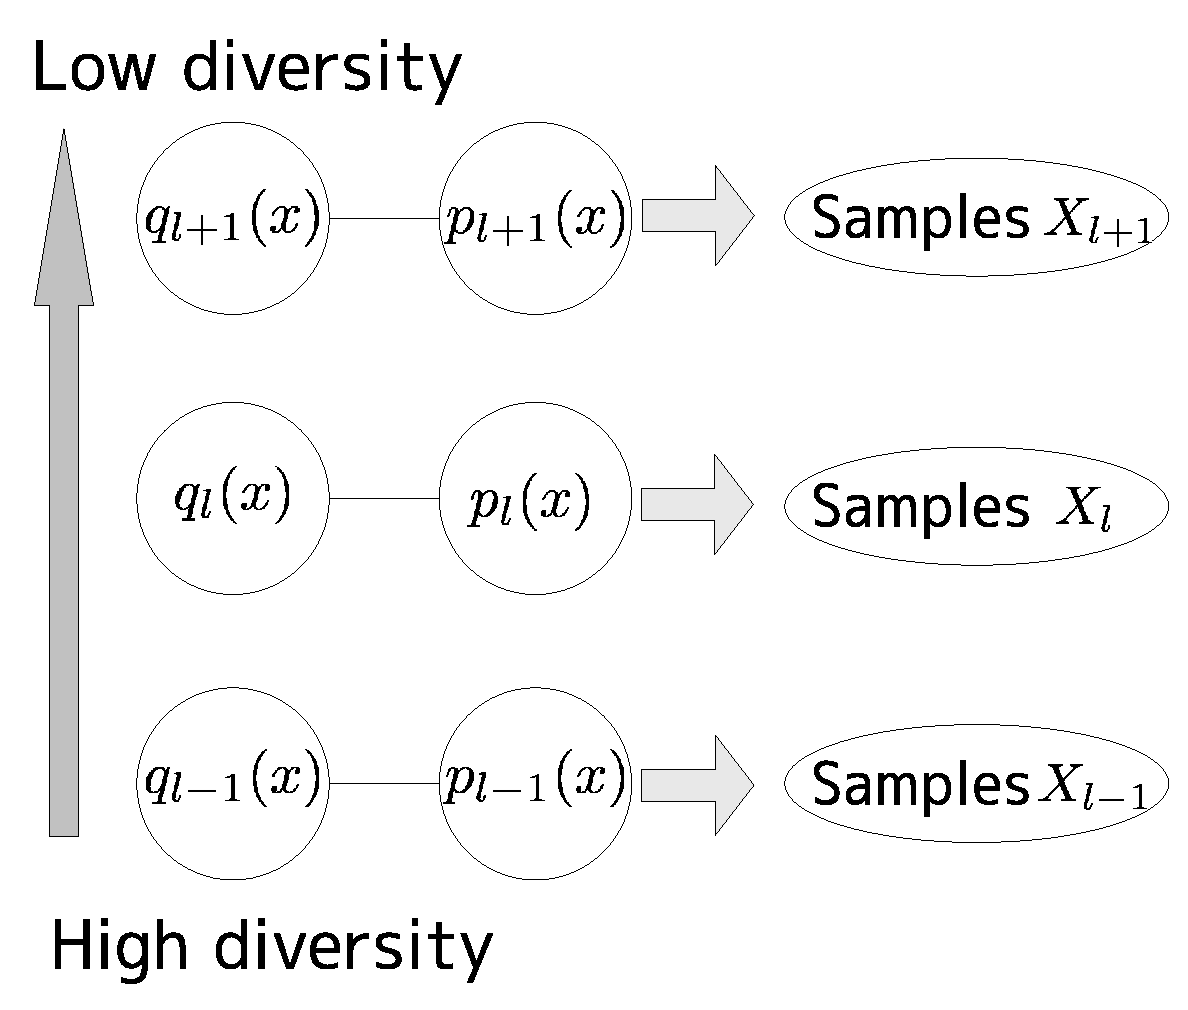
\includegraphics[width=\linewidth]{./data_his/his1.eps}}
\end{minipage}
&
\begin{minipage}{\linewidth}
\centerline{\includegraphics[width=\linewidth]{./data_his/his2.eps}}
\end{minipage}
\\
\spcen
(a) Sampling
&
\spcen
(b) Estimation
\\
\end{tabular}
\vskip -0.2in
\caption{Illustration of Hierarchical Importance Sampling.}
\label{fig-his}
\end{center}
\end{figure*}

\subsection{Comparison between HIS and the EAPM}
Suppose that the target distributions are previously provided in the EAPM and
HIS.
Let $L$ be the number of the layers of HIS.
At time $t$, the EAPM generates a probability model $p_t(x)$
approximating the corresponding target distribution $q_t(x)$,
whereas HIS generates 
$L$ number of probability models $p^{(t)}_0(x) \cdots p^{(t)}_{L-1}(x)$
approximating the corresponding target distributions 
$q_0(x) \cdots q_{L-1}(x)$, respectively.
To generate $p_t(x)$,
the EAPM uses only one sample set $X_{t-1}$, which is generated in the previous step.
On the other hand, to generate $p_l^{(t)}(x)$,
HIS uses all the sample sets $X_0^{(t-1)} \cdots X_{L-1}^{(t-1)}$,
generated in the previous step.
In other words, the difference is that
the EAPM sequentially generates probability models and sample sets,
whereas HIS generates probability models and sample sets
both simultaneously and iteratively.


If only the $l-1$th sample set $X_{l-1}$ is used
for updating the $l$th probability model $p_l(x)$ 
in the estimation step of HIS,
HIS, indeed, corresponds to iterative execution of the EAPM,
which means that the EAPM is restarted from the initialization
if the EAPM converges.
This implies that HIS is a mathematical extension of the EAPM.


\subsection{Target Distribution Control}
\label{sec-tdc}
HIS can theoretically operate
if the target distributions are previously defined in any manner.
However, in practice, HIS requires appropriate target distributions
to produce good results.
This section explains a manner in which 
the target distributions of HIS are provided.
Note that the proposed target distribution control method
in this section
cannot be directly applied with any probability distribution other than
 the partially uniform distribution defined by (\ref{pud}) 
for target distributions.
Further discussion is left in Chapter \ref{chapter-ers}.


It is supposed that $q_0(x)$ and $q_{L-1}(x)$ are given\footnote{
In the experiments, a probability distribution that generates only the
best obtained sample is used for $q_{L-1}(x)$.};
then the objective of the control method is
to determine $q_l(x)$ for $l=1 \cdots L-2$.
Each $q_l(x)$ is represented by the partially uniform distribution and
denoted by $q_l(x|\tilde f_l)$ 
with the threshold parameter $\tilde f$.
In terms of importance sampling,
$q_{l-1}(x)$ and the next target distribution $q_{l}(x)$ should be similar
because the accuracy of the empirical log-likelihood given by
the importance sampling depends on this similarity.
Thus, the objective is to select $\tilde f_l$ such that 
$q_{l-1}(x|\tilde f_{l-1})$, $q_l(x|\tilde f_l)$, and $q_{l+1}(x|\tilde f_{l+1})$ are similar.

The present concept is based on the size of the search space.
In the case of the partially uniform distribution,
a set of drawable samples is defined by 
\mbox{$C_l=\{x|\tilde q(x|\tilde f_l)=1\}$},
where $\tilde q(x|\tilde f)$ is defined by (\ref{truncation}),
and the number of drawable samples is given by
$
\int_C dx 
 = \int \tilde q(x) dx=Z
$.
Thus, the size of the search space can be provided by the
normalizing constant defined by (\ref{constant}).
Note that the normalizing constant is normally unknown,
but its estimator can be calculated through importance sampling as follows:
\begin{eqnarray}
Z_l(\tilde f) &=& \int \tilde q(x|\tilde f) dx \nonumber \\
 & \simeq & \frac{1}{M} \sum_{p(x)} \frac{\tilde q(x|\tilde
 f)}{p(x)} \nonumber \\
&=& \hat Z_l(\tilde f), \label{est-z}
\end{eqnarray}
where $\sum_{p(x)}$ denotes summation over the samples generated from
$q(x)$  and $M$ is the number of the samples.
In an importance sampling calculation,
\begin{equation}
\frac{1}{M}\sum_{{q_{l-1}(x)}} \frac{q_l(x)}{q_{l-1}(x)} f(x),\\
\end{equation}
the probability of generating an acceptable sample,
whose weight $\frac{q_{l}(x)}{q_{l-1}(x)}$ is not zero,
is given by 
\begin{equation}
 \int_{C_{l-1}} q_{l-1}(x) \frac{\tilde q_l(x)}{\tilde q_{l-1}(x)} dx=\frac{Z_l}{Z_{l-1}},
\end{equation}
where it is assumed that $C_l \subseteq C_{l-1}$.
It is clear that the rejected samples do not contribute
to the importance sampling.
In the EAPM under an assumption that samples are generated 
not from the probability models
but from the target distributions, 
the sum of the number of the accepted samples throughout the optimization
process
is given by
\begin{equation}
 \sum_{l=1}^{L-1} M_{l-1} \frac{Z_l}{Z_{l-1}},
\label{accept-samples}
\end{equation}
where $L$ is the number of iterations. 
The maximization condition of $Z_l$ with respect to
(\ref{accept-samples}) is given by
\begin{equation}
 M_{l-1}\frac{Z_l^*}{Z_{l-1}}=M_l \frac{Z_{l+1}}{Z_l^*},
\label{eq-tdc}
\end{equation}
where $Z_l^*$ is the optimal value.

If $Z_{l-1}$ and $Z_{l+1}$ are given\footnote{
Note that $Z_0$ and $Z_{L-1}$ are normally previously provided and thus,
all $Z_l$ can be previously determined according to (\ref{eq-tdc}).
However, this paper uses the estimators of $Z_{l-1}$ and $Z_{l+1}$
to determine $Z_l$ because, in some cases, it can be difficult to 
build a probability model approximating a target distribution with a
certain normalizing constant.},
the target normalizing constant $Z_l^{*}$ is obtained from (\ref{eq-tdc}).
Then, the threshold parameter $\tilde f_l$ is updated to
satisfy 
\begin{equation}
 Z_l^{*}=\hat Z_l(\tilde f_l),
\label{eq-threshold}
\end{equation}
where $\hat Z_l(\tilde f_l)$ is
the estimator of the normalizing constant given by (\ref{est-z}).
A method for solving (\ref{eq-threshold})
is described in Section \ref{sec-ftilde}. 
Figure \ref{search_space} shows an illustration of the
search space reduction.

\begin{figure}[tb]
\centerline{\includegraphics[width=\hfiglength\linewidth]{./data_his/searchspace.eps}}
\caption{Search Space Reduction.}
\label{search_space}
\end{figure}


\subsection{Practical Procedure}
In the practical procedure of HIS,
first of all, each $p_l(x)$
is initialized to a uniform distribution and
each $X_l$ is generated from $p_l(x)$.
For each $l$, the $l$th layer (i.e., $q_l(x)$, $p_l(x)$, and $X_l$) is
sequentially and iteratively updated.
To update the $l$th layer,
first, $q_l(x)$ is updated according to (\ref{eq-tdc}),
and then $p_l(x)$ is updated.
To calculate the empirical log-likelihood with respect to $q_l(x)$,
we use only three sample sets, which are the upper one $X_{l-1}$,
the current one $X_l$, and the lower one $X_{l+1}$\footnote{$X_{-1}$ and
$X_L$ are supposed to be null sets.}
for two reasons:
calculating the marginal probability (\ref{eq-mixture}) consumes a
considerable amount of time, and
the samples in $X_i$, generated from $p_i(x)$, tend not to contribute
to the importance sampling (\ref{mix-is})
if $p_i(x)$ and $q_l(x)$ are not similar.
Finally, the sample set $X_l$ is replaced with
samples newly generated from $p_l(x)$.
The pseudo-code of HIS
is shown in Fig. \ref{his-algo}.

\begin{figure}[t]
\renewcommand{\arraystretch}{1.23}
\centering
\begin{tabular}{lp{.9\linewidth}}
\multicolumn{2}{c}{Hierarchical Importance Sampling (HIS)}\\
\hline
1 & Initialize the probability models $p_0(x) \cdots p_{L-1}(x)$ and
the sample sets $X_0 \cdots X_{L-1}$.
$l \Leftarrow 0$.
\\
2 & do\{ \\
3 & ~~Adjust the target distribution $q_l(x)$ according to (\ref{eq-tdc}).\\
4 & ~~ \parbox[t]{.85\linewidth}{Calculate the empirical log-likelihood with
 respect to $q_l(x)$ from
 $X_{l-1},X_l,X_{l+1}$ through importance sampling according to (\ref{mix-is}).} \\
5 & ~~ \parbox[t]{.85\linewidth}{Update the probability model $p_l(x)$ according to
 the empirical log-likelihood.}\\
6 & ~~ \parbox[t]{.85\linewidth}{Generate samples from $p_l(x)$ and replace
the sample set $X_l$ with the generated samples.}\\
7 & ~~ $l \Leftarrow (l+1)\%L$.\\
8 & \}until(stopping criterion reached)\\
\hline
\end{tabular}
\vspace{3mm}
\caption{The Pseudo-code of Hierarchical Importance Sampling.}
\label{his-algo}
\end{figure}


\section{Experiments}
This section describes the experiments conducted to investigate
the advantages of HIS 
through comparison with EDA.


\subsection{Experimental Setup}
The present experiments are set up according to the experiments of
Section \ref{exp-rpm}.

\subsubsection{HIS Setting}
HIS employs the online updating defined in Section \ref{exp-rpm-setup}.
All the parameter settings are described as follows:
\begin{itemize}
 \item The number of generated samples in one sampling $M$ : $10$ or $50$.
 \item The number of the layers $L$: $10$, $20$, $30$, or $40$.
 \item Learning rate $\alpha$: 0.5.
\end{itemize}
These values are experimentally determined.
Note that the number of samples contained in $X_i$
is denoted by $M_i$ and $M_i=M_j=M$.


\subsection{Results}


%\newcommand{\spcen}{\centering \vskip 0.05in}

\begin{table}[tbp]
%\footnotesize
\centering
\caption{\tabletitle{HIS}{Onemax}}
%\vskip 0.05in
\begin{tabular}{|r|r|rr|rr|}
\hline
\multicolumn{1}{|c|}{Samples} & \multicolumn{1}{c|}{Cutoff} &
 \multicolumn{2}{c|}{Best} & 
 \multicolumn{2}{c|}{Evaluations}  \\ \hline
10 & 10 & --400 &  (0) & 29155 &  (12095.51) \\ \hline
10 & 20 & --400 &  (0) & 32743 &  (11000.43) \\ \hline
50 & 10 & --400 &  (0) & 48435 &  (20868.97) \\ \hline
10 & 30 & --400 &  (0) & 56170 &  (16627.74) \\ \hline
10 & 40 & --400 &  (0) & 67595 &  (20897.39) \\ \hline
50 & 20 & --400 &  (0) & 82215 &  (15277.81) \\ \hline
50 & 30 & --400 &  (0) & 113680 &  (23360.03) \\ \hline
50 & 40 & --400 &  (0) & 157715 &  (35272.9) \\ \hline
\end{tabular}
\label{his-onemax}
\end{table}

\begin{figure}[tbp]
\centering
\centerline{\includegraphics[width=\figlength\linewidth]{./data_his/his_1dising_s10.eps}}
(a) $M=10$\\
\vspace{0.1in}
\centerline{\includegraphics[width=\figlength\linewidth]{./data_his/his_1dising_s50.eps}}
(b) $M=50$
\caption{\tabletitle{HIS}{1D Ising}}
\label{his-1d-ising}
\end{figure}

\begin{figure}
\centering
\centerline{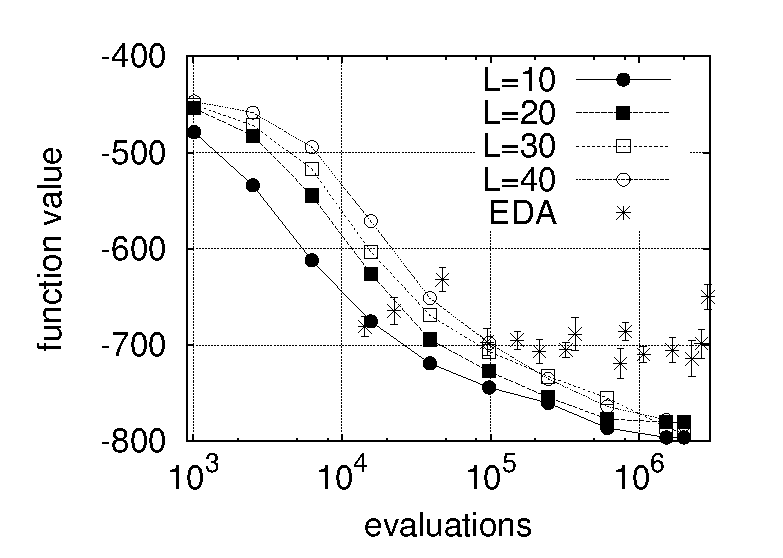
\includegraphics[width=\figlength\linewidth]{./data_his/his_2dising_s10.eps}}
(a) $M=10$ \\
\vspace{0.1in}
\centerline{\includegraphics[width=\figlength\linewidth]{./data_his/his_2dising_s50.eps}}
(b) $M=50$
\caption{\tabletitle{HIS}{2D Ising}}
\label{his-2d-ising}
\end{figure}

%\vskip 0.2in




Table \ref{his-onemax} shows the results of HIS for Onemax.
The first and the second columns list the number of generated samples
per sampling and the number of layers, respectively.
The third column lists the average cost function value,
 with the standard deviation
in parenthesis, of the best obtained solutions over ten independent runs.
The forth column lists the number of function evaluations.

Figures \ref{his-1d-ising} and \ref{his-2d-ising} show
the results of HIS for the 1D and 2D Ising models, respectively.
In each figure,
the horizontal axis represents the number of function evaluations,
while the vertical axis represents the average cost function value.
Each point represents the average cost function value of the best obtained
solutions over ten independent runs
for the corresponding number of function evaluations performed.
The standard deviations are negligibly small and may be ignored.
Additionally, the results of EDA are appended for comparison.
The points correspond to the results in
Tables \ref{ann-1d-ising} or \ref{ann-2d-ising}
in Appendix \ref{exp-edace}.

The results for Onemax show that
HIS performs as well as EDA.
For EDA, $M$ should be set at more than $100$;
otherwise, EDA can not find the optima.
Figures \ref{his-1d-ising} and \ref{his-2d-ising}
show that HIS can find better solutions than EDA.
EDA may exhibit faster convergence than HIS;
however, given sufficient time 
(i.e., a sufficient number of function evaluations), 
HIS can find better solutions than EDA.


\section{Discussion}
\subsection{Escaping Local Optima}
As shown in Figs. \ref{his-1d-ising} and \ref{his-2d-ising},
it is clear that HIS can afford better solutions than EDA.
The number of samples employed by HIS for building a probability model
is given by
\begin{equation}
 3 \times M.
\end{equation}
The number of samples that EDA uses for building a probability model
is given by
\begin{equation}
 (1-c) \times M.
\end{equation}
When $M=10$, HIS uses $30$ samples; on the other hand,
when $M=100$ and $c=0.3$, EDA uses  $70$ samples.
This implies that HIS can escape from local optima
by using fewer samples.

In EDA and the EAPM,
the entropy of the target distribution
is decreased in a stepwise fashion and
the target distribution is tracked 
by a probability model.
For tracking the target distribution,
the expected log-likelihood must be estimated.
The accuracy of an estimator of the expected log-likelihood 
is dependent on the accuracy of the approximation of the probability model.
Thus, once an inferior probability model is built,
the accuracy of the estimator of the log-likelihood 
with respect to the next target distribution is also compromised.
Subsequently, 
acceptable probability models cannot be generated.  
This phenomenon can be understood as dropping into local optima.

On the other hand,
HIS overcomes this problem by maintaining 
multiple probability models.
In HIS, the larger is the entropy of a target distribution,
the easier it is to approximate it.
More specifically,
low layers tend to have good probability models
and high layers tend to have bad probability models.
HIS iteratively improves the probability models in the higher layers 
with samples generated from the lower layers.
Thus, if the lower layers have good probability models,
the expected log-likelihood can be
estimated well at the layers above them.
Once a good probability model is built,
it tends not to make a change for the worse.
Consequently,
HIS sequentially improves all the probability models 
from the lowest layer.
 
\subsection{Iterative EDA}
\begin{figure}[tbp]
\begin{center}
\begin{tabular}{p{\hfiglength\linewidth}p{\hfiglength\linewidth}}
\begin{minipage}{\linewidth}
\centerline{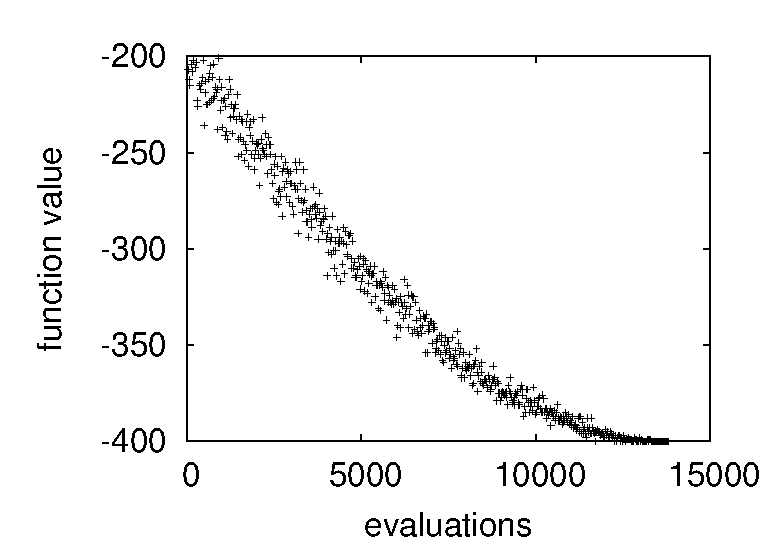
\includegraphics[width=\linewidth]{data_his/annealing_graph.eps}}
\end{minipage}
&
\begin{minipage}{\linewidth}
\centerline{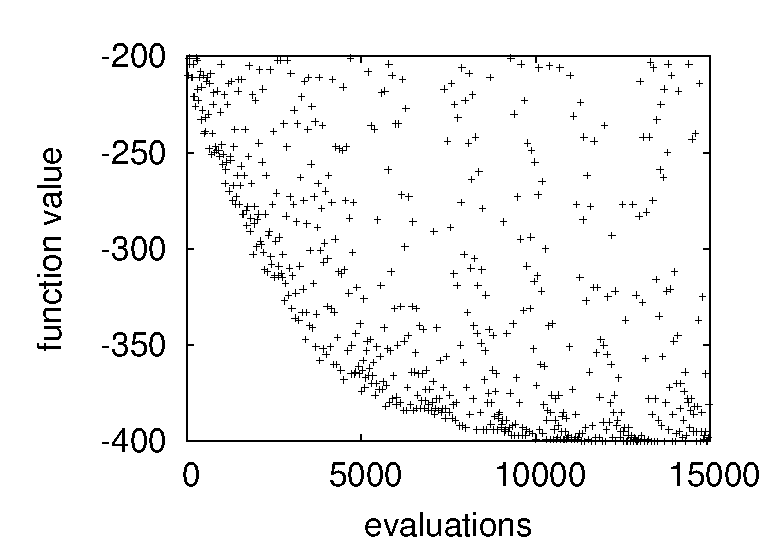
\includegraphics[width=\linewidth]{data_his/his_graph.eps}}
\end{minipage}
\\
\spcen
(a) EDA
&
\spcen
(b) HIS
\\
\end{tabular}
\vskip -0.2in
\caption{Optimization Process of EDA ($M=100, c=0.3$) and 
HIS ($L=10,M=10$) 
for 400-dimensional Onemax.}
\label{fig-process}
\end{center}
\end{figure}

The more the number of function evaluations performed, 
the better the solutions afforded by HIS. 
This is because the samples generated by HIS always have certain diversity.
Figure \ref{fig-process} shows
the cost function values of the samples generated by HIS and EDA.
The horizontal axis represents the number of function evaluations, while
the vertical axis represents the cost function value.
HIS has no convergence, and therefore, can find the optimum solution
eventually.
However, this is not an unique advantage of HIS
because no convergence can also be realized by iterative EDA.

As the results of EDA for 1D Ising and 2D Ising show,
iterative EDAs do not perform as well as HIS
because the standard deviations of the best values are insufficiently small.
For example, the $10$ best obtained solutions in $100$ trials
of EDA with $M=3000$ and $c=0.5$ for the 2D Ising 
are $-746$, $-736$, $-732$, $-732$, $-730$, $-730$, $-730$,
$-728$, $-726$, and  $-726$.
If the target distributions are assumed to be previously provided,
HIS is an extension of the EAPM.
The advantage of HIS
is the use of the samples and probability models of other trials, 
whereas each trial in iterative EDA is independently executed.

\subsection{Parameters}
In sampling-based optimization,
there exists a trade-off between
the number of function evaluations and 
the quality of the obtained solutions.
In other words,
the greater is the number of function evaluations,
the better are the solutions afforded.
In EDA, the number of function evaluations perfomed 
until convergence depends on
the parameters: the number of generated samples in one sampling and
the cutoff rate.
If a solution with a certain quality is needed,
it becomes necessary to provide good parameters.

On the other hand,
HIS does not converge, and
the best obtained value is gradually improved.
Thus, it can be said that the setting of the parameters in HIS
is easier than in EDA. 
However, both the number of function evaluations necessary and
the efficiency of HIS depend on the number of layers.
A greater number of layers in HIS
affords greater similarity 
between adjacent target distributions (i.e., $q_l(x)$ and
$q_{l-1}(x)$), implying that 
it is easier for HIS with a greater number of layers 
to escape from local optima.
On the other hand, HIS with a greater number of layers 
requires more function evaluations 
because the samples generated from bad probability models
are useless, and the probability models in the higher layers 
tend to be bad at the early stages.
The number of layers may be expected to be determined adaptively
according to the accuracy of the probability models:
this will be the subject of future work.

\subsection{Computational Cost}
HIS can provide better results,
but at greater computational cost than EDA.
First, HIS requires $L$ times the memory space required by EDA:
$L$ number of probability models and 
$L$ number of sample sets maintained in HIS. 
Second, HIS consumes greater computational time than EDA:
the calculation of the probability of the mixture distribution
given by (\ref{eq-mixture}) requires considerable time.

\subsection{Mixture Model-based EDAs}
In terms of using a mixture distribution,
some mixture model-based EDAs such as
\cite{pelikan:mixture} can be considered similar works.
However, they are classified as methods with annealing
because they simply split samples generated from one probability
model into a number of groups and
gradually converge each group,
whereas HIS organizes the diversity of all the probability models.
Thus, the optimization process of them is almost equivalent to
one illustrated in  Fig. \ref{fig-process}-(a).

Note that HIS can simply employ a mixture distribution as the
probability model of each target distribution.
In terms of statistical estimation,
the model error can be reduced by using a mixture model.
On the other hand, HIS improves the accuracy
of the empirical log-likelihood in terms of importance sampling.


\subsection{Comparison with Markov Chain Monte Carlo}
\label{app-mcmc}

Calculating the expectation with respect to the distribution of interest
is common to 
Markov chain Monte Carlo methods (MCMC) \cite{bishop:ml} and EAPM.
Table \ref{eda-mcmc} briefly shows the relationship between
MCMC and EAPM.

The key concepts behind MCMC are local transition,
which realizes effective sampling,
and designing it as a
Markov chain by satisfying {\it detailed balance}, 
which guarantees mathematical validity.
On the other hand,
the principle feature of EAPM is estimating 
an effective probability distribution
and sampling from it.
The mathematical validity is guaranteed by importance sampling.

In the practical methods, there exist correspondence relations.
For example, simulated annealing (SA) \cite{kirkpatrick:sa} corresponds to
general EDA and the EAPM in terms of sequentially tracking a target distribution, 
and the exchange Monte Carlo method 
(EMC) \cite{hukushima:emc} corresponds to HIS 
in terms of sampling from multiple target distributions.

\begin{table}[tbp]
\centering
\caption{MCMC and EDA.}
\vskip \tableskiplength
\begin{tabular}{|c|c|c|}
\hline
 &MCMC & EAPM\\ \hline
Mathematical Validity & Detailed Balance & Importance Sampling \\ \hline 
Effective Sampling & Local Transition & Estimated Probability Model \\ \hline
Sequential & SA & the EAPM \\ \hline
Parallel & EMC & HIS \\ \hline
\end{tabular}
\label{eda-mcmc}
\end{table}


\section{Summary}
This chapter proposed Hierarchical Importance Sampling (HIS),
a method that can be used instead of the annealing
for the EAPM.
Experimental comparisons between HIS and EDA revealed that
HIS outperforms EDA.
The advantages of HIS can be summarized as follows:
(1)it affords better solutions than EDA
by escaping from local optima, 
and (2)it allows the parameters to be set easily.